\chapter[Referencial Teórico]{Referencial Teórico}

Para dar início ao referencial teórico de forma concisa e alinhada ao que foi apresentado no Capítulo 1, é fundamental abordar o contexto e o papel da Fertilização In Vitro, a qualidade dos embriões e os principais desafios envolvidos nesse processo. Além disso, é essencial evidenciar como técnicas de Aprendizado de Máquina, com destaque para as Redes Neurais Artificiais, podem contribuir para o aprimoramento das taxas de sucesso da gravidez, a mitigação de riscos relacionados a abortos e alterações cromossômicas, bem como a redução dos impactos emocionais e físicos enfrentados por pacientes submetidas a esse tipo de tratamento.

\section{Fertilização In Vitro}

A fertilidade tem sido um tema de grande relevância ao longo da história humana, visto como uma bênção divina em diversas culturas. Civilizações antigas, como a grega e a egípcia, realizavam rituais, usavam amuletos e talismãs, ou buscavam ajuda de divindades para garantir a continuidade de suas linhagens e prosperidade \cite{moura2020}. Esses métodos, embora enraizados em crenças religiosas e espirituais, refletem o desejo universal de superar desafios relacionados à reprodução.

Com os avanços científicos e médicos, a compreensão da fertilidade passou por uma profunda transformação. O primeiro marco da inseminação artificial em humanos ocorreu em 1978, com o nascimento de Louise Brown, o primeiro "bebê de proveta" \cite{moura2020}. Este feito foi possível graças ao desenvolvimento da técnica de Fertilização In Vitro (FIV), criada pelo embriologista Robert Edwards e pelo ginecologista Patrick Steptoe. A técnica permitiu a fertilização de embriões fora do corpo humano e, por sua contribuição revolucionária, Edwards recebeu o Prêmio Nobel de Fisiologia ou Medicina em 2010 \cite{corleta2010}.

As Técnicas de Reprodução Assistida (TRA) compreendem um conjunto de métodos médicos especializados que buscam ajudar indivíduos com dificuldades reprodutivas a alcançarem a concepção \cite{souzamarise2024}. Dentre essas técnicas, a FIV se destaca como a mais avançada e amplamente utilizada \cite{moura2020}. O processo envolve várias etapas, como a estimulação ovariana controlada (uso de medicamentos para estimular a produção de óvulos), coleta de óvulos por punção transvaginal, fertilização em laboratório e posterior transferência dos embriões formados para o útero \cite{moura2020}.

Além de estabelecer as bases da medicina reprodutiva moderna, o nascimento de Louise Brown abriu caminho para avanços na medicina reprodutiva. Desde então, a combinação de avanços médicos e tecnológicos permitiu não apenas a realização da fertilização in vitro, mas também a análise genética detalhada dos embriões \cite{moura2020}. Esses exames identificam anomalias cromossômicas e genéticas, proporcionando uma maior chance de sucesso na implantação e no desenvolvimento de gestações saudáveis.

Os esforços históricos e as inovações científicas ilustram a busca contínua da humanidade por soluções eficazes contra a infertilidade. No próximo tópico, discutiremos detalhadamente a análise de embriões, um procedimento crucial para aumentar as chances de concepção saudável e seu papel na e seu papel na seleção de embriões para a FIV.

\section{Métodos de Avaliação Genética em Reprodução Assistida}

No contexto das Tecnologias de Reprodução Assistida, os métodos de avaliação genética desempenham um papel essencial na identificação de anomalias cromossômicas, como a aneuploidia, que é a alteração no número normal de cromossomos da espécie humana, representa a principal causa de falhas de implantação quando sua origem é embrionária. Dessa forma, a presença de aneuploidia nas células do embrião pode impactar diretamente a taxa de sucesso das técnicas de reprodução humana assistida. Além de dificultar a implantação, essa alteração cromossômica pode levar a abortos espontâneos ou até mesmo a malformações em bebês nascidos vivos \cite{milanezi2022}. Após décadas de avanços científicos, os testes genéticos tornaram-se cada vez mais precisos, com o desenvolvimento de técnicas sofisticadas e integradas à tecnologia, como a Testagem Genética Pré-implantacional.

Pelo final do século XX, o método do PGT começou a ser usado para realizar o rastreamento de doenças genéticas que possuíam uma alta taxa de incidência nas populações de amostra \cite{yang2024}. Com ele, foi propiciada a triagem de embriões antes da implantação, permitindo a seleção de embriões que possuíam menos riscos \cite{yang2024}. Tais métodos incluem a Testagem Genética Pré-implantacional para Doenças Monogênicas (PGT-M), como distrofia miotônica e fibrose cística; para rearranjos estruturais cromossômicos (PGT-SR); para aneuploidias (PGT-A), como Síndrome de Down e Síndrome de Turner; e mais recentemente, o PGT-P para doenças poligênicas \cite{yang2024}. No caso do nosso objeto de estudo, PGT-A, se destaca por sua capacidade de aumentar as chances de implantação embrionária bem-sucedida, reduzir a probabilidade de perdas gestacionais espontâneas e garantir maior probabilidade de nascimento de crianças com o número de cromossomos normais\cite{yang2024}. Além disso, o embrião considerado “normal” (euploide) apresenta 23 pares de cromossomos (46 cromossomos no total), sendo metade proveniente do espermatozoide e metade do óvulo. Já o embrião “anormal” (aneuploide) possui uma contagem incorreta de cromossomos em uma célula, sendo a maioria dos embriões com aneuploidias não compatíveis com a vida \cite{zegers2017}.

Os testes genéticos realizados durante a fase de blastocisto, formados cerca de 5{–}6 dias após a inseminação \cite{zegers2017}, são geralmente preferidos por especialistas em reprodução assistida porque essa abordagem envolve a coleta de células do trofectoderma, a camada externa do embrião que futuramente dará origem à placenta e não diretamente do interior do embrião \cite{leaver2019}. Essa técnica, o PGT-A, é considerada menos invasiva em comparação com as biópsias realizadas na fase de clivagem, quando o embrião possui apenas algumas células e está em um estágio muito inicial de desenvolvimento \cite{leaver2019}. Na fase de clivagem, a retirada de células do interior do embrião (blastômeros), pode causar danos mais significativos ao embrião, afetando sua capacidade de se desenvolver adequadamente e reduzindo as chances de implantação bem-sucedida no útero \cite{leaver2019}. 

No entanto, é fundamental mencionar que a técnica de micromanipulação necessária para realizar esses procedimentos ainda não foi completamente padronizada. Isso significa que diferentes laboratórios podem adotar práticas distintas para a biópsia embrionária, o que pode resultar em variações na segurança e eficácia dos testes. Além disso, os impactos potenciais dessa intervenção, tanto nos desfechos reprodutivos (como taxas de gravidez e nascimento) quanto na saúde a longo prazo dos bebês nascidos a partir desses embriões, ainda não estão completamente compreendidos.

O PGT-A classifica os embriões em três categorias: euploide (normal, com 46 cromossomos), mosaico (mistura de células normais e anormais) e aneuploide (todas as células com número anormal de cromossomos). 
%A Figura~\ref{fig:ResultadosPGT} ilustra os resultados do PGT-A e suas respectivas probabilidades de sucesso gestacional.

\begin{center}
    \begin{figure}[h]
        \captionsetup{font=footnotesize, position=above}
        \caption{Resultados do PGT-A e suas respectivas probabilidades de sucesso gestacional}
        \label{fig:ResultadosPGT}
        \centering
        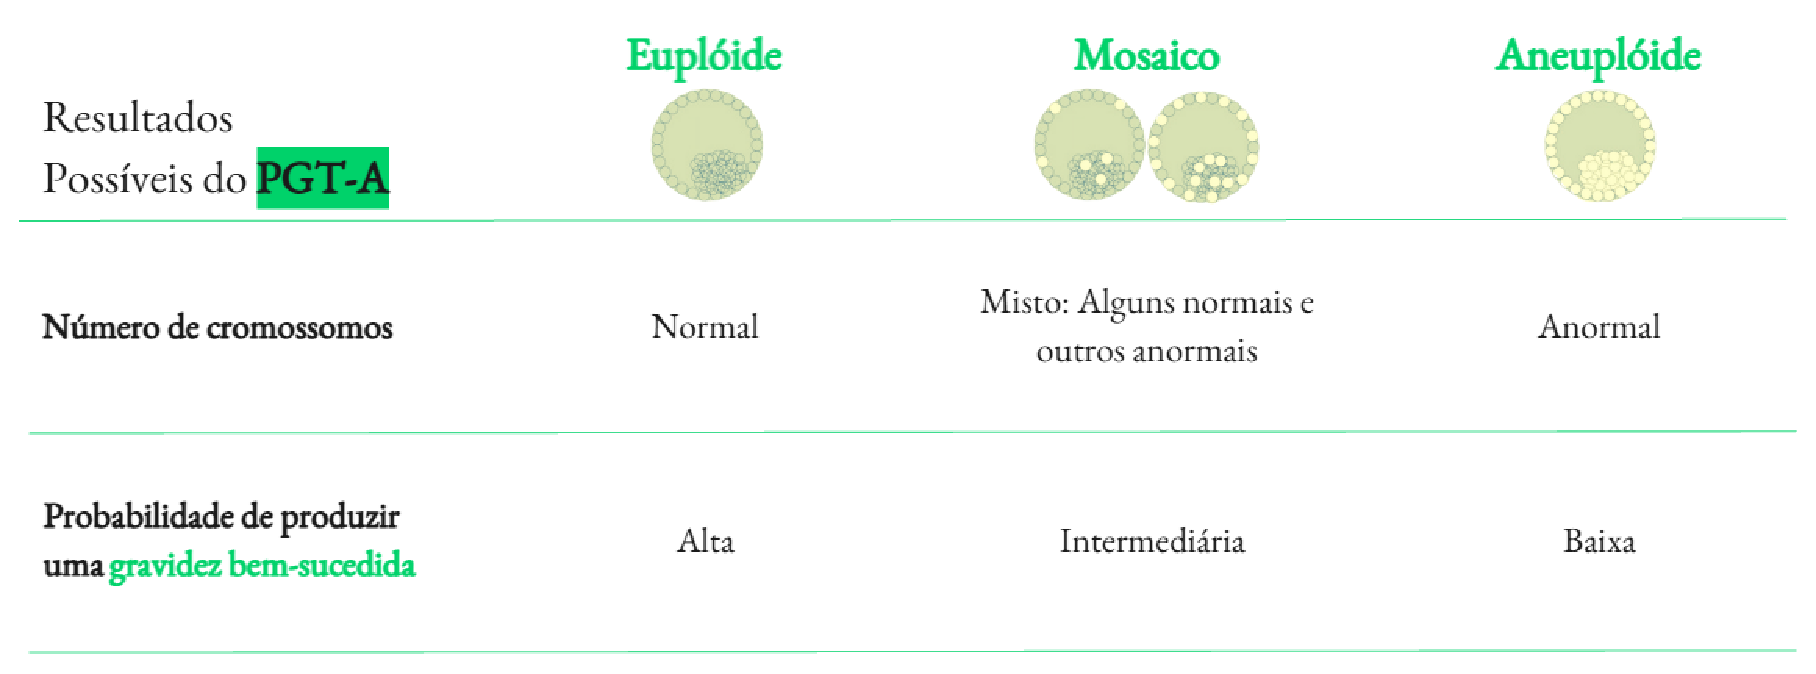
\includegraphics[scale=0.5]{figuras/ResultadosPGT.pdf}
        \vspace{0.3cm} 
        % \caption{Classificação dos embriões após o teste genético pré-implantacional para aneuploidias (PGT-A). O PGT-A avalia o número de cromossomos em células do embrião, permitindo classificá-los em três categorias: euploides (número normal de cromossomos), mosaicos (mistura de células com número normal e anormal de cromossomos) e aneuploides (número anormal de cromossomos em todas as células). A figura ilustra esquematicamente as diferentes classificações e as respectivas probabilidades de sucesso gestacional.}
        % \scriptsize{Classificação dos embriões após o teste genético pré-implantacional para aneuploidias (PGT-A). O PGT-A avalia o número de cromossomos em células do embrião, permitindo classificá-los em três categorias: euploides (número normal de cromossomos), mosaicos (mistura de células com número normal e anormal de cromossomos) e aneuploides (número anormal de cromossomos em todas as células). A figura ilustra esquematicamente as diferentes classificações e as respectivas probabilidades de sucesso gestacional.}
    \end{figure}
\end{center}
\FloatBarrier

Apesar de suas vantagens, o PGT-A apresenta limitações significativas, como a variabilidade nos resultados das biópsias do trofectoderma e o risco de diagnósticos falso-positivos \cite{gleicher2021}. A The Preimplantation Genetic Diagnosis International Society (PGDIS) e a European Society of Human Reproduction and Embryology (ESHRE) apontam questões críticas, incluindo:

\begin{itemize}
    \item As divergências no conteúdo de DNA aneuploide entre diferentes regiões da trofoectoderma e a massa celular interna demonstram que a biópsia de cinco células pode apresentar resultados variados;
    \item O número exato de células na biópsia nunca é conhecido, o que impossibilita determinar com precisão a porcentagem de DNA aneuploide;
    \item A biópsia da trofoectoderma danifica células individuais, causando vazamento de DNA e contaminação das células vizinhas, dificultando a medição precisa da aneuploidia;
    \item O limiar de 20\% entre euploidia e mosaicismo é baseado apenas na sensibilidade atual do sequenciamento de nova geração (NGS), que não detecta níveis inferiores a 20\% de DNA aneuploide. Consequentemente, qualquer mosaicismo abaixo de 20\% é considerado euploide normal;
    \item Dentro da faixa de mosaicismo (20\% a 80\%), os desfechos de implantação e nascimento são semelhantes, indicando que o uso de limiares rígidos para predizer resultados de FIV é incorreto.
\end{itemize}

Estudos indicam que embriões descartados como aneuploides pelo PGT-A resultaram em nascimentos normais \cite{gleicher2021}, evidenciando a necessidade de revisar as diretrizes para evitar o desperdício de embriões viáveis. A figura abaixo ilustra a seleção de um pedaço do embrião e como isso pode influenciar a definição da ploidia do mesmo. A biópsia mencionada nas etapas do PGT-A, envolvendo a remoção de uma célula do embrião para análise genética. \citeonline{phillips2024}, levantam a preocupação de que a remoção dessas células em crescimento possa comprometer o desenvolvimento do embrião, afetando os resultados neonatais, visto que as técnicas de micromanipulação utilizadas na biópsia não são totalmente isentas de riscos, como observado por \citeonline{leaver2019}.

\begin{figure}[h]
    \captionsetup{font=footnotesize, position=above}
    \caption{Discrepância potencial entre uma biópsia de células utilizando PGT-A e a composição celular em regiões adjacentes do trofectoderma}
    \label{fig:biopsiaPGT-A}
    \centering
    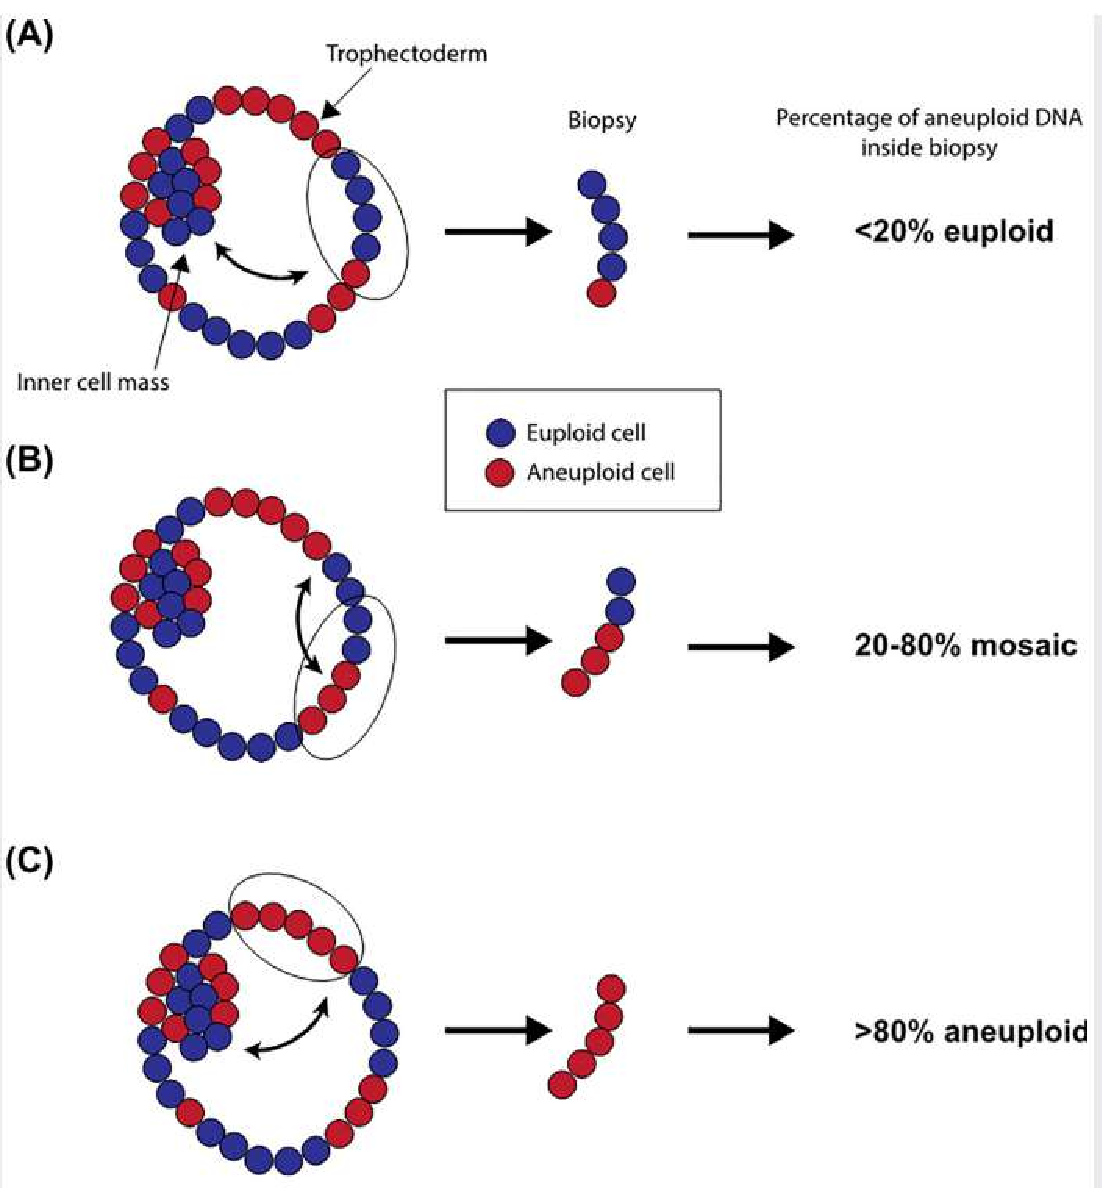
\includegraphics[scale=0.6]{figuras/biopsiaPGT-A.pdf}
    \vspace{0.3cm} 
    \begin{minipage}{\linewidth}
        \centering
        % \caption{Representação esquemática da biópsia do trofectoderma e a influência da amostragem na determinação da ploidia embrionária. (A) Embrião euploide com células da massa celular interna (MCI) e do trofectoderma (TE) com pouca ou nenhuma aneuploidia. A biópsia resulta em uma amostra com menos de 20\% de células aneuploides, classificando o embrião como euploide. (B) Embrião mosaico com proporção similar de células euploides e aneuploides. A biópsia pode resultar em uma amostra com 20-80\% de células aneuploides, classificando o embrião como mosaico. (C) Embrião predominantemente aneuploide. A biópsia resulta em uma amostra com mais de 80\% de células aneuploides, classificando o embrião como aneuploide. Observação: A ploidia embrionária determinada pela biópsia do trofectoderma pode variar de acordo com a região amostrada, devido à mosaicidade embrionária. A figura ilustra a incerteza associada à classificação da ploidia embrionária com base em uma pequena amostra de células.}
        % \scriptsize{Representação esquemática da biópsia do trofectoderma e a influência da amostragem na determinação da ploidia embrionária. (A) Embrião euploide com células da massa celular interna (MCI) e do trofectoderma (TE) com pouca ou nenhuma aneuploidia. A biópsia resulta em uma amostra com menos de 20\% de células aneuploides, classificando o embrião como euploide. (B) Embrião mosaico com proporção similar de células euploides e aneuploides. A biópsia pode resultar em uma amostra com 20-80\% de células aneuploides, classificando o embrião como mosaico. (C) Embrião predominantemente aneuploide. A biópsia resulta em uma amostra com mais de 80\% de células aneuploides, classificando o embrião como aneuploide. Observação: A ploidia embrionária determinada pela biópsia do trofectoderma pode variar de acordo com a região amostrada, devido à mosaicidade embrionária. A figura ilustra a incerteza associada à classificação da ploidia embrionária com base em uma pequena amostra de células.}
    \end{minipage}
\end{figure}
\FloatBarrier

Embora o PGT-A permita detectar aneuploidias e aumente as chances de uma gravidez bem-sucedida, ele pode impactar negativamente o potencial de implantação do embrião \cite{gleicher2021}. Por esses motivos, métodos não invasivos estão sendo estudados como alternativas eficientes e seguras, tornando-se cada vez mais relevantes. Um exemplo de técnica não invasiva é a análise morfocinética a partir de imagens obtidas de incubadoras de última geração equipadas com a tecnologia Time-Lapse System.

\section{Time-Lapse System}

O TLS é um sistema que captura imagens contínuas dos embriões em desenvolvimento, em intervalos regulares, sem alterar o ambiente de cultivo \cite{moustakli2024}. Essa análise morfocinética, gerada pelas imagens adquiridas pelo TLS, permite o monitoramento quase contínuo do desenvolvimento do embrião, possibilitando a observação de eventos dinâmicos e frequentemente transitórios que não seriam visíveis em observações estáticas \cite{boucret2021}. O uso do TLS não interrompe as condições de cultura, mantendo a viabilidade do embrião durante o processo de monitoramento \cite{moustakli2024}.

As variáveis morfocinéticas incluem aspectos como a forma e a estrutura do embrião (morfológicas) e o movimento e o desenvolvimento do embrião ao longo do tempo (cinéticas), os quais são essenciais para uma análise detalhada de seu progresso \cite{gleicher2021}. Com esse monitoramento contínuo, é possível observar a regularidade das divisões celulares e identificar momentos críticos do crescimento, o que pode auxiliar na diferenciação de embriões euplóides e aneuplóides com base no seu padrão de desenvolvimento \cite{boucret2021}. De acordo com \citeonline{moustakli2024}, o TLS oferece insights valiosos sobre a saúde e o potencial de desenvolvimento dos embriões, utilizando uma abordagem não invasiva, em contraste com a biópsia de embriões. Alguns estudos indicam que, ao ser combinado com pontuações morfocinéticas, o TLS pode aumentar as taxas de implantação e gravidez clínica em comparação aos métodos tradicionais \cite{boucret2021}.

As variáveis da planilha de dados, dados esses extraídos pelo TLS, que estamos utilizando para esse trabalho incluem informações sobre a qualidade morfológica e cinética dos embriões, como a taxa de divisão celular e a regularidade do desenvolvimento. Essas variáveis são essenciais para a análise morfocinética e a classificação dos embriões em diferentes estágios de desenvolvimento \cite{boucret2021}. A seguir, discutiremos as variáveis cientificamente comprovadas que influenciam a ploidia.

\subsection{Idade}

As informações trazidas pelo Fertility and Ageing (\citeonline{eshre2005}) corroboram a relevância de incluir variáveis relacionadas à \textbf{idade materna}, pois estudos apontam que o aumento da aneuploidia em embriões está diretamente associado ao envelhecimento materno. O estudo de \citeonline{yuan2023} aponta que a taxa de euploidia dos embriões está correlacionada com a idade feminina. À medida que a idade avança, há um declínio no número total e na qualidade dos ovócitos, um fator crítico para a fecundidade reduzida observada após os 35 anos \cite{yuan2023}.

\subsection{t2, t3, t4, t5, t8, s2, cc2 (t3-t2), tSC, tSB, tB, cc3 (t5-t3), s3 (t8-t5), t5-t2,  tSC-t8 e tB-tSB}

Os \textbf{sistemas de Time-Lapse} ajudam a identificar \textbf{marcadores morfocinéticos}, que mostram como as células se dividem durante o desenvolvimento do embrião. Esses marcadores, junto com características físicas tradicionais, são fundamentais para selecionar o embrião mais adequado para a transferência \cite{souzarebeca2022}. O desenvolvimento embrionário é um processo dinâmico, com mudanças perceptíveis em um curto período \cite{cruz2012}. Estudos detalhados sobre o ritmo das divisões celulares, assim como características como tamanho e organização das células, demonstram que o tempo necessário para atingir certos estágios de desenvolvimento está diretamente relacionado ao potencial de implantação do embrião \cite{souzarebeca2022}.

Embriões que se dividem muito rapidamente apresentam menor chance de implantação quando comparados aos que seguem um ciclo celular dentro do intervalo considerado normal \cite{cruz2012}. Isso acontece porque mudanças no tempo que o embrião leva para se desenvolver nas primeiras fases estão ligadas a uma maior chance de problemas genéticos no número de cromossomos \cite{cruz2012}. O projeto \textit{Timing of cell division in human cleavage-stage embryos is linked with blastocyst formation and quality} de \citeonline{cruz2012} utilizou o sistema Time-Lapse para identificar marcadores morfocinéticos e monitorar com precisão os tempos das divisões celulares durante o desenvolvimento embrionário. Os tempos considerados ótimos para previsões de desenvolvimento embrionário foram: \textbf{t2 (24,3{–}27,9 horas), t3 (35,4{–}40,3 horas), t5 (48,8{–}56,6 horas), s2 (<0,76 horas) e cc2 (<11,9 horas)}. A explicação detalhada dessas variáveis está disponível no \textbf{Apêndice \ref{apendice:variaveis}}.

Especificamente, no nível morfológico, \textbf{t5} destacou-se como o indicador mais relevante do potencial de implantação \cite{cruz2012}. Observa-se que a capacidade de diferenciar embriões viáveis daqueles não viáveis melhora significativamente quando os critérios se baseiam em eventos de divisão celular mais tardios \cite{cruz2012}. Embriões com t5 entre 48,8 e 56,6 horas demonstram não apenas um maior potencial de implantação, mas também uma maior propensão a se desenvolverem em blastocistos de morfologia superior \cite{cruz2012}.

Ao criar um modelo de IA para a previsão de euploidia, é importante que considere as variáveis \textbf{t4, t8, tSC, tSB, tB, cc3 (t5 - t3) e s3 (t8 - t5)}. Essas métricas são fundamentais para o desenvolvimento embrionário, conforme evidenciado no estudo que comprovou a efetividade da IA em detectar embriões viáveis com uma precisão de 70\% \cite{rienzi2020}. A incorporação dessas variáveis em um modelo de IA é crucial, pois possibilita a captura das sutilezas do desenvolvimento embrionário, que, de acordo com a pesquisa, são melhoradas através da análise automatizada fundamentada em Inteligência Artificial. Isso se torna especialmente relevante pois os sistemas de time-lapse disponibilizam informações detalhadas e contínuas, que podem ser combinadas para detectar padrões relacionados à euploidia \cite{rienzi2020}.

A avaliação de fatores morfocinéticos, como o tempo necessário para clivagem e a extensão das fases subsequentes, tem sido alvo de pesquisa para antecipar a probabilidade de implantação embrionária. Por exemplo, um estudo publicado pelo Instituto Sapientiae por \citeonline{desai2019} destacou a importância desses parâmetros na predição do potencial de implantação embrionária. Apesar dessa pesquisa não tratar especificamente os intervalos \textbf{t5-t2, tSC-t8 e tB-tSB}, ela sugere que a avaliação de intervalos de tempo entre eventos específicos no desenvolvimento embrionário pode oferecer percepções valiosas sobre a qualidade e a capacidade de desenvolvimento dos embriões \cite{desai2019}.

\subsection{Estágio e Morfo}

Modelos de IA têm sido empregados na avaliação de embriões produzidos até o quinto dia ou mais, com o objetivo de aprimorar a escolha com base em informações objetivas e de alta exatidão \cite{lassen2022}. Esses modelos priorizam a análise dos estágios "\textbf{Dia 5+}", ou seja, aqueles que atingem o estágio de blastocisto no quinto dia ou mais tarde, devido à maior disponibilidade de dados morfológicos e dinâmicos do desenvolvimento embrionário \cite{lassen2022}. 

De acordo com os critérios definidos por \citeonline{gardner1999}, com base na \textbf{morfologia do embrião} se tem a categorização dos blastocistos, um fator determinante para o potencial de implantação e a qualidade embrionária \cite{capalbo2014}. Os blastocistos são agrupados em quatro categorias principais, considerando tanto a massa celular interna (ICM, Inner Cell Mass) quanto o TE (trophectoderma):
\begin{itemize}
  \item \textbf{Grupo 1 (Excelente)}: Blastocistos com classificação  \textbf{$\geq$ 3AA}. Blastocistos altamente desenvolvidos com massa celular interna densa e trophectoderma bem organizado \cite{capalbo2014}.
  \item \textbf{Grupo 2 (Bom)}: Blastocistos com classificação \textbf{3, 4, 5 ou 6} e com notas \textbf{AB ou BA}. Apresentam características boas, mas menos consistentes em relação ao grupo excelente \cite{capalbo2014}.
  \item \textbf{Grupo 3 (Médio)}: Blastocistos com classificação \textbf{3, 4, 5 ou 6} e notas \textbf{BB, AC ou CA}. Qualidade moderada com irregularidades tanto na ICM quanto no TE \cite{capalbo2014}.
  \item \textbf{Grupo 4 (Ruim)}: Blastocistos com classificação \textbf{$\leq$ 3BB}.Blastocistos de menor qualidade, com poucas células organizadas na ICM e TE menos coeso \cite{capalbo2014}.
\end{itemize}
O estudo de \citeonline{capalbo2014} enfatizou a relação entre a morfologia padrão dos blastocistos, a euploidia e as taxas de implantação. Blastocistos de excelente morfologia, particularmente os biopsiados no dia 5, mostraram uma maior probabilidade de serem euploides e apresentaram taxas de implantação superiores.

\subsection{KIDScore\texttrademark}  

O KIDScore\texttrademark{}, um algoritmo baseado em IA aplicado à análise de imagens em sistemas Time-Lapse, tem se mostrado uma ferramenta importante na avaliação de embriões durante os tratamentos de reprodução assistida \cite{kato2021}. O algoritmo combina variáveis morfocinéticas e parâmetros de desenvolvimento embrionário para fornecer uma pontuação que auxilia na seleção de embriões com maior potencial de implantação e viabilidade genética \cite{gazzo2020}. A pontuação vai de \textbf{0 a 10}. Pontuações baixas, entre 0 e 3, indicam embriões de qualidade inferior, com baixo potencial de implantação. Pontuações médias, de 4 a 6, correspondem a embriões de qualidade moderada, com um potencial razoável de implantação. Já pontuações altas, de 7 a 10, representam embriões de alta qualidade, com grande potencial de implantação \cite{gazzo2020}. \citeonline{kato2021} cita que o modelo apresentou uma alta precisão na previsão de resultados de gravidez, sendo especialmente útil tanto em pacientes com idade materna avançada quanto em pacientes mais jovens. Por fim, \citeonline{gazzo2020} informaram que o uso do algoritmo no processo de seleção embrionária levou a um aumento expressivo nas taxas de implantação após a transferência de embriões congelados (FET). Então o modelo quando combinada com informações sobre os tempos de divisão celular, sendo \textbf{t2, t3, t5, s2 e cc2} descritos por \citeonline{cruz2012}, possibilita um exame mais completo do crescimento embrionário, melhorando a acurácia na seleção de embriões com maior probabilidade de êxito em tratamentos de FIV.

\subsection{Ploidia}
Para a elaboração do nosso modelo de previsão de euploidia, optamos por empregar a coluna de \textbf{Ploidia}, que proporciona uma categorização minuciosa dos embriões em diversas categorias de euploidia. As categorizações contidas nesta coluna são: Aneuploide complexo, Aneuploide/Triploide XXX, Caótico, Haploide, Mosaico de alto grau, Mosaico de baixo grau e Normal/Euploide. De acordo com o \citeonline{bastida2019}, considera-se os embriões com Caótico, Haplóide e Mosaico de alto grau como Aneuploides, enquanto os com mosaico de baixo grau como Euploides. Diante disso, optamos por reorganizar os valores na tabela de dados, agrupando as seguintes categorias sob o termo \textbf{Aneuploide}: Aneuploide complexo, Aneuploide/Triploide XXX, Caótico, Haploide e Mosaico de alta complexidade. Em contrapartida, os embriões categorizados como Mosaico de baixo grau e Normal/Euploide serão reunidos na categoria \textbf{Euploide}.

\section{Aprendizado de Máquina}

As dificuldades em definir IA não são, portanto, o resultado de alguma deficiência ou descuido, mas surgem do fato de que fomos incapazes de determinar precisamente qual inteligência desejaríamos replicar artificialmente \cite{sheikh2023}. Dessa forma, definimos a Inteligência Artificial como sistemas que exibem comportamento inteligente ao analisar seu ambiente e tomar ações, com algum grau de autonomia, para atingir objetivos específicos \cite{sheikh2023}. 

Na medicina reprodutiva, a IA tem se mostrado promissora na melhoria de processos como a fertilização in vitro (FIV). Essa busca por imitar a inteligência humana e entender seus processos cognitivos levou ao desenvolvimento de diversas abordagens, entre elas o Aprendizado de Máquina (Machine Learning, ML), que envolve a capacidade de computadores de interpretar grandes volumes de dados, construir modelos baseados nesses dados e, assim, gerar hipóteses ou previsões sobre o mundo ao seu redor \cite{russell2016}. Na medicina, algoritmos podem ser treinados para reconhecer padrões genéticos em embriões, classificar o melhor embrião para implantação e prever características genéticas de novos embriões. 

Os métodos de ML são geralmente classificados em três tipos principais: aprendizado supervisionado, aprendizado não supervisionado e aprendizado por reforço. Neste estudo, opta-se pelo aprendizado supervisionado como abordagem principal, dada sua eficácia na análise de dados rotulados, permitindo decisões mais precisas e embasadas para otimizar os tratamentos de FIV.

O aprendizado supervisionado consiste no treinamento de algoritmos com base em conjuntos de dados rotulados, nos quais as variáveis de entrada (inputs) e os resultados esperados (outputs) já são conhecidos. O algoritmo aprende a correlacioná-los de forma eficiente \cite{russell2016}, ajustando seus parâmetros com base nas diferenças entre previsões e resultados reais \cite{trask2019}. Uma técnica amplamente usada dentro do aprendizado supervisionado é a classificação, cujo objetivo é atribuir rótulos ou classes pré-definidas aos dados. Por exemplo, no contexto da medicina reprodutiva, um modelo pode ser treinado para diferenciar embriões euploides e aneuploides, aprendendo a reconhecer padrões associados a cada grupo \cite{izbicki2020}.

\begin{figure}[h]
    \captionsetup{font=footnotesize, position=above}
    \caption{Aprendizado Supervisionado: Identificando Euploidia e Aneuploidia}
    \label{fig:biopsiaPGT-A}
    \centering
    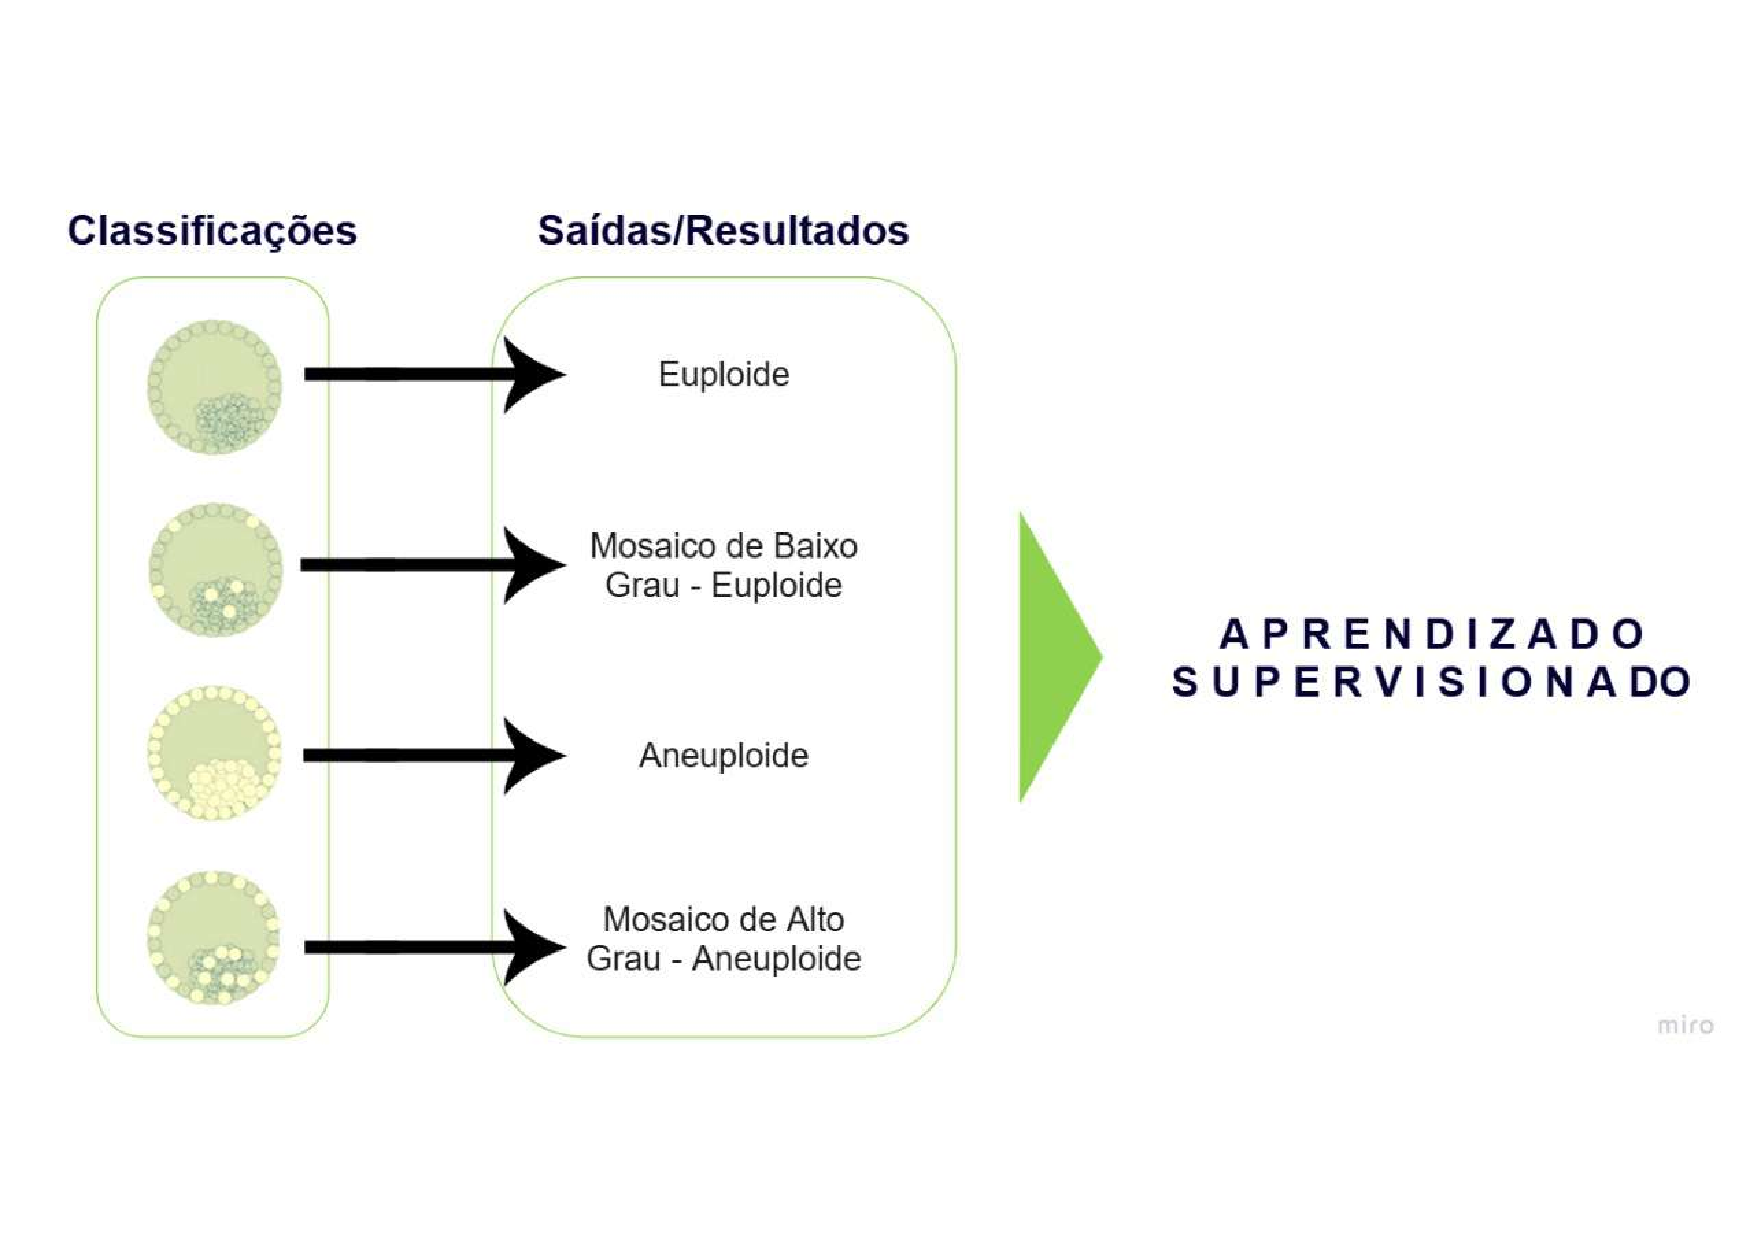
\includegraphics[scale=0.35]{figuras/aprendizadoSuper.pdf}
    \vspace{0.3cm} 
    % \caption{Os dados já possuem seus próprios rótulos. Já é definido o que significa ser euploide e aneuplóide. Os dados rotulados (ou seja, com rótulos já atribuídos) são usados para treinar o modelo. Nesse contexto, ao se referir a "euploide" e "aneuplóide", esses rótulos podem representar classes que o modelo deve aprender a identificar com base nas características dos dados, ajudando a prever ou classificar novos casos com precisão.}
\end{figure}
\FloatBarrier

De maneira geral, um algoritmo de aprendizado supervisionado separa o banco de dados em três subconjuntos: treinamento, validação e teste \cite{izbicki2020}. Na fase de treinamento, o algoritmo identifica padrões nos dados de entrada e os associa às classes desejadas \cite{izbicki2020}. Na validação, um subconjunto de dados não utilizado no treinamento avalia o desempenho do modelo \cite{izbicki2020}, permitindo ajustes nos hiperparâmetros. Após resultados satisfatórios, o conjunto de testes mensura métricas como acurácia, recall e precisão, garantindo o desempenho esperado \cite{izbicki2020}.

A seleção aleatória das amostras para treinamento, validação e teste é uma boa prática \cite{izbicki2020}, evitando problemas decorrentes de ordenações previamente estabelecidas nos bancos de dados. Isso assegura uma visão representativa e imparcial dos dados, fundamental para a construção de modelos robustos e confiáveis \cite{izbicki2020}. 

Para a exploração inicial, utilizaremos as Redes Neurais Artificiais (RNAs) como alternativa metodológica. De acordo com \citeonline{haykin2009}, as RNAs são estruturas computacionais compostas por unidades de processamento simples, interconectadas, capazes de armazenar conhecimento adquirido por meio da experiência e aplicá-lo em novas situações. Além disso, o autor destaca que as redes neurais se assemelham ao cérebro humano em dois aspectos fundamentais: o conhecimento é adquirido a partir da interação com o ambiente por meio de um processo de aprendizado e esse conhecimento é armazenado nas conexões entre as unidades de processamento, chamadas de pesos sinápticos

Outro ponto de destaque é a capacidade de generalização das RNAs, ou seja, a habilidade do modelo de fornecer respostas coerentes para dados que não foram apresentados durante o treinamento. Segundo \citeonline{haykin2009}, essa propriedade permite que as redes neurais sejam aplicadas em problemas de alta complexidade, onde as relações entre as variáveis não são facilmente modeladas por técnicas convencionais, que é o nosso caso. Considerando a complexidade dos dados deste projeto, que incluem informações clínicas, morfológicas e morfocinéticas de embriões humanos, a aplicação de Redes Neurais Artificiais se mostra adequada, oferecendo maior potencial de precisão na predição da saúde genética dos embriões em tratamentos de FIV.

\subsection{Redes Neurais Artificiais (RNA)}

As Redes Neurais Artificiais (RNA) são modelos computacionais inspirados no funcionamento do cérebro humano, compostas por unidades chamadas neurônios artificiais interconectados. Essas redes têm a capacidade de aprender a partir de dados, capturando relações complexas e não lineares \cite{haykin2009}.

Segundo \citeonline{haykin2009}, uma Rede Neural Artificial (RNA) pode ser compreendida como um processador distribuído em larga escala, formado por unidades simples de processamento, que possui uma notável aptidão para armazenar conhecimento adquirido por meio da experiência e utilizá-lo posteriormente. Essa estrutura se assemelha ao cérebro humano em dois aspectos fundamentais: o conhecimento é adquirido a partir de um processo de aprendizado e armazenado por meio dos pesos sinápticos que conectam os neurônios artificiais. O objetivo fundamental de uma RNA é aproximar uma função desconhecida, relacionando um conjunto de entradas $x = (x_1, x_2, \ldots, x_n)$ a uma saída $y$, por meio da combinação ponderada dos sinais de entrada, processados em múltiplas camadas \cite{haykin2009}. Essa capacidade torna as redes neurais adequadas para tarefas como classificação, regressão, reconhecimento de padrões e outras aplicações que envolvam problemas com alta complexidade e não-linearidade.

As RNAs geralmente são organizadas em camadas: uma camada de entrada, uma ou mais camadas ocultas e uma camada de saída. Cada camada é composta por neurônios artificiais interligados, e os sinais de entrada percorrem essas camadas, sendo processados até gerar o resultado final. A forma como os neurônios estão interconectados e como os pesos são ajustados determina o desempenho do modelo \cite{haykin2009}. Dentre as arquiteturas mais conhecidas, destaca-se o Perceptron de Múltiplas Camadas (MLP), que, segundo \citeonline{haykin2009}, representa uma extensão do Perceptron original e se mostrou fundamental para o avanço das redes neurais, especialmente ao possibilitar a resolução de problemas complexos como o XOR, que não são solucionáveis por modelos lineares simples.

\subsubsection{Multilayer Perceptron (MLP)}

O Multilayer Perceptron (MLP) é uma das arquiteturas mais clássicas de Redes Neurais Artificiais (RNA) e consiste em uma rede feedforward (tipo de rede neural onde o fluxo de informações ocorre em apenas uma direção, da camada de entrada para as camadas ocultas e, finalmente, para a camada de saída, sem ciclos ou conexões retroativas), totalmente conectada, organizada em camadas sequenciais: uma camada de entrada, uma ou mais camadas ocultas e uma camada de saída \cite{haykin2009}. Cada neurônio em uma camada recebe entradas da camada anterior, aplica um somatório ponderado seguido de uma função de ativação não linear e transmite o resultado para a próxima camada. A camada de entrada é formada por n neurônios, onde cada neurônio representa uma variável do problema. As camadas ocultas são densamente conectadas, contendo respectivamente m e p neurônios, responsáveis por transformar e extrair representações cada vez mais abstratas dos dados. A camada de saída é composta por um único neurônio, que gera a probabilidade de pertencimento a uma das classes, no caso, a classificação do embrião como euploide ou aneuploide. As setas representam as conexões sinápticas entre os neurônios de cada camada, indicando o fluxo de processamento dos dados. A figura abaixo ilustra um MLP típico com uma camada de entrada, duas camadas ocultas e uma camada de saída.

\begin{figure}[h]
    \captionsetup{font=footnotesize, position=above}
    \caption{Estrutura de um MLP com uma camada de entrada, três camadas ocultas e uma camada de saída.}
    \label{fig:biopsiaPGT-A}
    \centering
    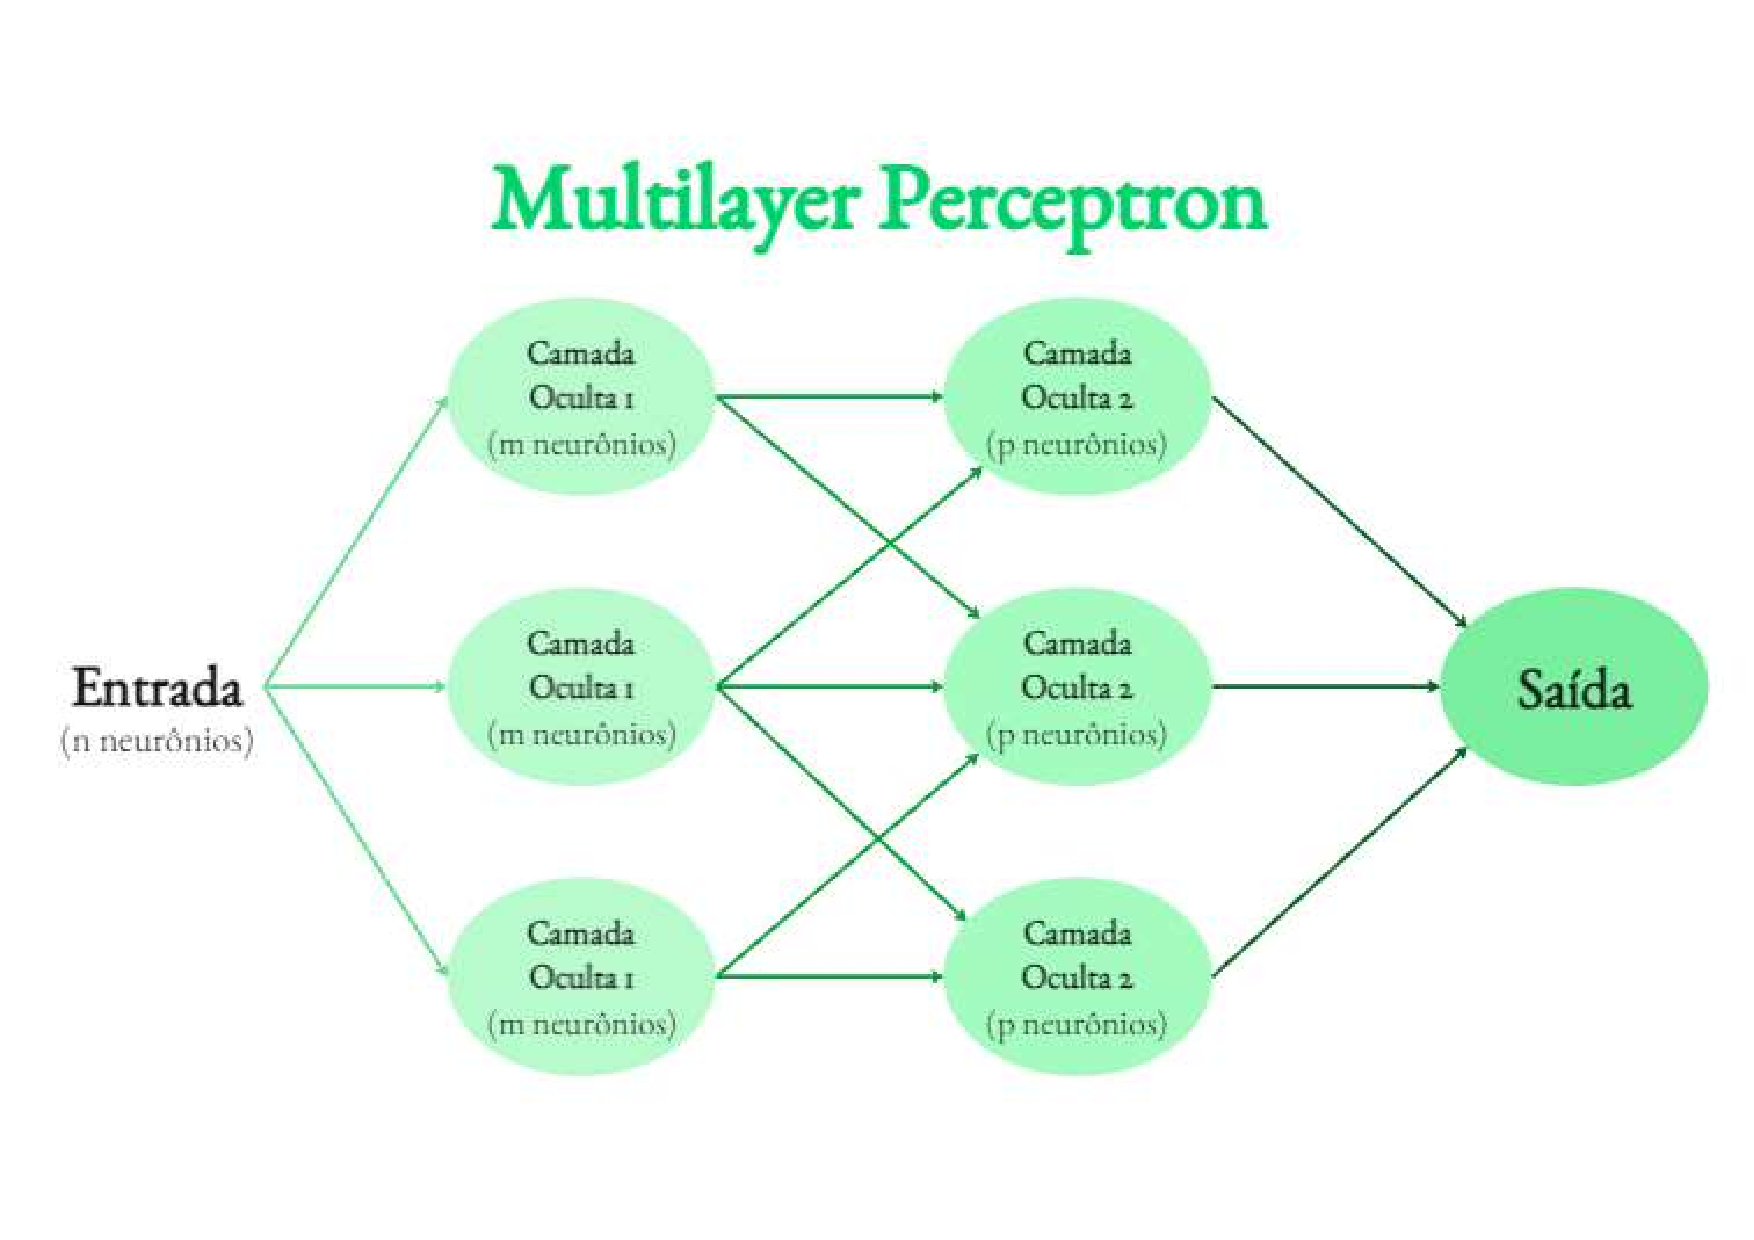
\includegraphics[scale=0.35]{figuras/multilayer.pdf}
    \vspace{0.3cm}
\end{figure}
\FloatBarrier

A principal função das camadas ocultas é extrair e transformar características relevantes dos dados, permitindo que a rede modele funções complexas e não lineares \cite{haykin2009}. No MLP que utilizaremos neste trabalho, serão configuradas duas camadas ocultas com 64 e 32 neurônios, respectivamente, buscando um equilíbrio entre capacidade de representação e eficiência computacional.

\subsubsection{Características das Camadas Densas}

As camadas do MLP são chamadas densas (\textit{fully connected}) porque cada neurônio em uma camada está conectado a todos os neurônios da camada seguinte. Essa estrutura permite que a rede aprenda combinações complexas dos atributos de entrada \cite{haykin2009}.

O cálculo realizado por um neurônio em uma camada densa pode ser expresso como:

\begin{equation}
    z = \sum_{i=1}^{n} w_i x_i + b
\end{equation}

Onde wi representam os pesos ajustáveis, xi as entradas e b o termo de viés bias. Em seguida, aplica-se uma função de ativação z, resultando na saída do neurônio:

\begin{equation}
    a = \phi(z)
\end{equation}

\subsubsection{Inteligência Artificial Explicável (XAI) e o Algoritmo LIME}

As Redes Neurais Artificiais (RNAs), especialmente aquelas com múltiplas camadas ocultas, são frequentemente classificadas como modelos de caixa-preta (black-box models). Essa denominação decorre do fato de que, apesar de sua notável capacidade de generalização e precisão preditiva, o processo interno que leva à tomada de decisão não é diretamente acessível ou interpretável por seres humanos \cite{adadi2018}. Isso ocorre devido à sua estrutura altamente complexa, composta por milhares, ou até milhões, de parâmetros ajustáveis, como pesos sinápticos, vieses e funções de ativação, distribuídos ao longo de diversas camadas ocultas. Como resultado, ainda que um modelo baseado em RNA indique que determinado embrião possui alta probabilidade de ser euploide, não é possível saber com clareza quais atributos ou relações entre variáveis motivaram essa predição \cite{ribeiro2016}.

Em domínios sensíveis, como a medicina reprodutiva, essa falta de transparência representa um risco considerável. À medida que algoritmos de aprendizado de máquina são cada vez mais utilizados para auxiliar na tomada de decisões clínicas, torna-se imprescindível que seus resultados sejam não apenas precisos, mas também explicáveis. É nesse cenário que se insere a área de Inteligência Artificial Explicável (XAI {–} Explainable Artificial Intelligence), cujo propósito é desenvolver métodos que permitam compreender o raciocínio subjacente às decisões dos modelos de aprendizado de máquina \cite{gilpin2018}. A XAI visa, portanto, mitigar o tradicional trade-off entre desempenho e interpretabilidade, viabilizando a aplicação segura e confiável de modelos complexos em contextos que exigem responsabilidade, rastreabilidade e validação técnica e ética das decisões automatizadas \cite{gilpin2018}.

Essa necessidade é ainda mais crítica quando se considera que a arquitetura não linear das RNAs impossibilita a extração de regras explícitas ou justificativas lógicas que expliquem suas predições de forma direta. Assim, surge um questionamento fundamental: é aceitável confiar em sistemas cujas decisões não podem ser auditadas ou compreendidas? No campo da saúde, em especial, a ausência de explicações pode comprometer a adoção dessas tecnologias por profissionais clínicos, reguladores e pacientes. A confiança em sistemas baseados em IA vai além da acurácia estatística — ela requer transparência sobre os critérios e evidências que fundamentam cada recomendação.

Para contornar essa limitação, diversas técnicas de XAI foram desenvolvidas. Entre as mais difundidas está o LIME (Local Interpretable Model-Agnostic Explanations), algoritmo proposto por Ribeiro, Singh e Guestrin (2016). O LIME é classificado como agnóstico ao modelo, pois pode ser aplicado a qualquer tipo de preditor, seja ele uma árvore de decisão, um modelo de ensemble ou uma rede neural profunda, sem a necessidade de conhecer sua estrutura interna ou lógica computacional específica.

O princípio do LIME consiste em gerar explicações locais para decisões individuais, em vez de tentar interpretar o funcionamento global do modelo. Para isso, o algoritmo realiza amostragens perturbativas na entrada a ser explicada — pequenas variações nos valores das variáveis de entrada — e observa como o modelo responde a essas modificações \cite{ribeiro2016}. Com base nessa vizinhança artificial gerada, o LIME ajusta um modelo explicativo simples (como uma regressão linear com regularização) que simula o comportamento do modelo original apenas naquela região local do espaço de entrada. Os coeficientes obtidos por esse modelo linear representam, portanto, a importância relativa de cada atributo para a decisão observada \cite{ribeiro2016}.

Essa abordagem será utilizada no presente trabalho com o objetivo de explicar as predições do modelo MLP treinado para estimar a probabilidade de um embrião ser euploide. Ao aplicar o LIME, será possível calcular a contribuição percentual de cada variável para cada embrião, tornando o processo de decisão mais transparente e confiável. A utilização de ferramentas de XAI como o LIME agrega valor clínico ao modelo de predição, permitindo uma análise interpretável dos fatores morfocinéticos envolvidos na determinação da euploidia.

\section{Identificação de Padrões Morfocinéticos e Predição de Euploidia com IA e Trabalhos Correlatos}

Os dados que são coletados pela tecnologia do TLS, são chamados de “dados morfocinéticos”, que são definidos como dados do desenvolvimento dos embriões \cite{moustakli2024}. Essa informação reunida proporciona noções detalhadas sobre o padrão do desenvolvimento e divisão celular embrionário. Atualmente, após recorrentes estudos sobre esses dados, sabe-se que as características morfocinéticas dos embriões têm sido associadas à avaliação de sua potência de desenvolvimento, ou seja, se um embrião analisado pelo TLS tenha um melhor desenvolvimento, ele terá mais probabilidade de ser euplóide, pois um bom desempenho de um embrião é capaz de prever a implantação \cite{yuan2023}. 

Os modelos de TLS, de acordo com \citeonline{yuan2023}, tem uma avaliação contínua na etapa do desenvolvimento embrionário por meio de suas imagens e, por observações estáticas, monitora as características do embrião, como tempo e padrões de divisão celular, fornecendo uma base para prever a euploidia. O TLS por si só, não opera com a IA, mas é frequentemente mesclado com essa tecnologia para maiores análises. Um exemplo é o estudo do \citeonline{yuan2023}, o artigo “Development of an artifcial intelligence based model for predicting the euploidy of blastocysts in PGT‐A treatments” o qual teve como objetivo utilizar o TLS e desenvolver um modelo de IA usando uma técnica de regressão logística, para predizer a euploidia de blastocistos—fase do desenvolvimento embrionário que ocorre após a clivagem do óvulo fertilizado—em tratamentos de PGT-A, ajudando a identificar embriões com maiores possibilidades de serem geneticamente normais antes da etapa de transferência. O modelo foi avaliado com uma boa precisão, indicando que ele consegue distinguir entre embriões euploides e aneuploides.

Outro estudo é o de \citeonline{souzarebeca2022}, “Análise da ploidia de embriões humanos por meio da inteligência artificial com o uso de variáveis de morfologia, morfocinética e variáveis relacionadas com a paciente”, que também utiliza IA, mas combinando dados morfológicos, morfocinéticos e clínicos para prever a ploidia dos embriões, utilizando uma rede neural artificial para classificá-los como euploides ou aneuploides. Em contraste, o modelo proposto neste projeto busca prever a porcentagem de aneuploidia, oferecendo uma análise quantitativa detalhada, em vez de uma classificação binária. Essa abordagem visa proporcionar uma compreensão mais profunda da saúde genética dos embriões, permitindo decisões mais precisas durante a seleção. 

Divergente do trabalho de \citeonline{yuan2023} e de \citeonline{souzarebeca2022}, que focam na predição binária de euploidia (ou seja, identificar se um embrião é euploide ou aneuploide), o modelo proposto neste projeto visa prever a porcentagem de aneuploidia dos embriões. Essa abordagem oferece um indicador quantitativo em vez de uma simples classificação binária, permitindo uma análise mais detalhada e informativa sobre a saúde genética dos embriões. Com isso, embriologistas poderão avaliar não apenas se um embrião é geneticamente normal, mas também entender o grau de aneuploidia presente, possibilitando decisões mais precisas durante o processo de seleção.

Além disso, nosso modelo busca ser uma alternativa menos invasiva e mais acessível. Embora técnicas atuais, como o PGT-A (Testagem Genética Pré-implantacional), forneçam informações precisas sobre a euploidia, elas dependem de métodos invasivos, como a biópsia embrionária, e de infraestrutura avançada, o que pode limitar o acesso a essas tecnologias em algumas clínicas. Com o uso de IA e dados de morfocinética obtidos via TLS (Time-Lapse System), o objetivo é desenvolver uma solução que permita uma avaliação robusta sem a necessidade de procedimentos invasivos, ampliando o alcance e a aplicação da tecnologia.

Um exemplo de modelo amplamente utilizado na prática clínica é o \textit{KIDScore\texttrademark{} Day 5} , que classifica embriões com base no seu potencial de implantação, sendo frequentemente usado em dispositivos como o \texttrademark{}\cite{reignier2019}. Esse modelo utiliza grandes bancos de dados multicêntricos para atribuir uma pontuação ao embrião, ajudando a ranquear os embriões do mesmo ciclo, facilitando a escolha do embrião com maior potencial para transferência \cite{reignier2019}.

Apesar dos avanços e do sucesso clínico do KIDScore\texttrademark{}, algumas limitações importantes foram destacadas na literatura. Segundo \citeonline{reignier2019}, o desempenho desses modelos pode ser influenciado por variáveis como idade materna, número de oócitos, origem dos oócitos e características específicas de cada centro de FIV, como as condições de  embrionária e uso de oxigênio reduzido. Isso destaca a necessidade de criar modelos robustos fundamentados em grandes conjuntos de dados multicêntricos e amplamente representativos, a fim de assegurar maior generalização e confiabilidade nos resultados.

Dentro desse cenário, o sistema CHLOE\texttrademark{} (Cultivating Human Life through Optimal Embryos), desenvolvido pela Fairtility\texttrademark{}, se destaca como uma ferramenta inovadora no campo da FIV por usar IA e visão computacional para prever com precisão a implantação e o desenvolvimento dos blastocistos. \cite{chole}. Enquanto nosso modelo é mais quantitativo e menos invasivo, o CHLE oferece uma solução mais integrada e transparente, visando otimizar a seleção de embriões de formas complementares, com foco na acurácia e confiança no processo de FIV  Essa tecnologia utiliza análises baseadas em imagens, o que indica um método não invasivo, além de oferecer uma análise transparente das decisões tomadas pela IA \cite{chole}.

De forma semelhante ao CHLOE\texttrademark{}, nosso modelo também combina IA e dados morfocinéticos para oferecer uma avaliação robusta e detalhada dos embriões. No entanto, enquanto o CHLOE\texttrademark{} se destaca por sua integração e foco na confiança do processo, nosso modelo propõe uma abordagem que enfatiza a estimativa quantitativa da porcentagem de aneuploidia, permitindo uma análise ainda mais detalhada da qualidade genética dos embriões. 

Com essas similaridades e diferenças em mente, nosso objetivo é desenvolver um modelo preditivo que combine precisão e acessibilidade, oferecendo uma análise quantitativa detalhada da saúde genética dos embriões. Essa abordagem tem o potencial de melhorar as taxas de sucesso nos tratamentos de fertilização in vitro, contribuindo para decisões mais informadas e eficazes no processo de seleção embrionária.